\documentclass{beamer}
\usepackage[english]{babel}
\usepackage{amsmath,amssymb,graphicx}

%%%%%%%%%% Start TeXmacs macros
\catcode`\<=\active \def<{
\fontencoding{T1}\selectfont\symbol{60}\fontencoding{\encodingdefault}}
\newcommand{\nospace}{}
\newcommand{\tmfoldedstd}[2]{\trivlist{\item[$\bullet$]\mbox{}#1}}
\newcommand{\tmmathbf}[1]{\ensuremath{\boldsymbol{#1}}}
\newenvironment{itemizedot}{\begin{itemize} \renewcommand{\labelitemi}{$\bullet$}\renewcommand{\labelitemii}{$\bullet$}\renewcommand{\labelitemiii}{$\bullet$}\renewcommand{\labelitemiv}{$\bullet$}}{\end{itemize}}
%%%%%%%%%% End TeXmacs macros

\begin{document}

{\screens{\begin{frame}
  \
  
  \
  
  \
  
  \
  
  \
  
  \title{计算视觉与模式识别}
  
  \maketitle
  
  \ 
\end{frame}}{\begin{frame}
  \frametitle{立体视觉}
  
  \resizebox{1\columnwidth}{!}{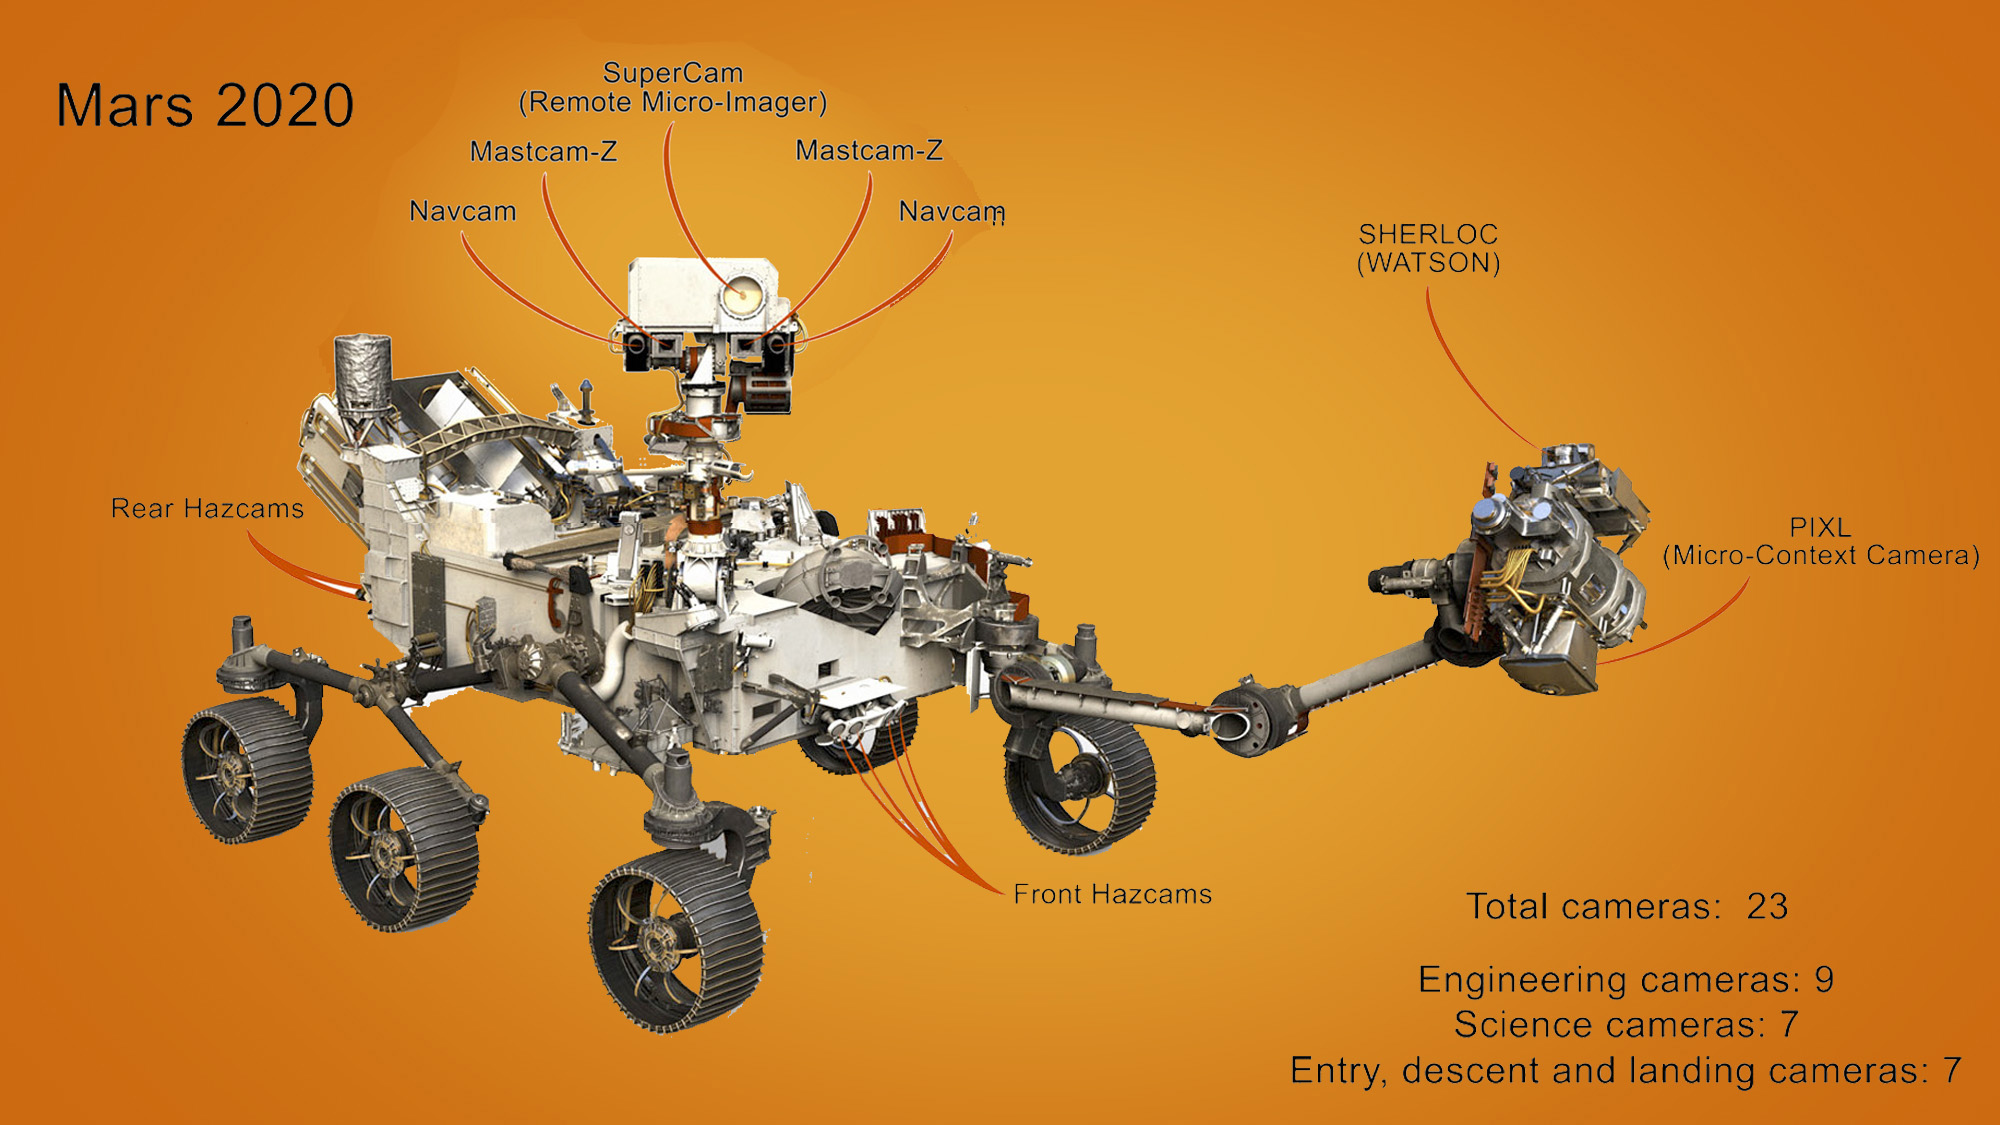
\includegraphics{img/mars2020.png}}
\end{frame}}{\begin{frame}
  \frametitle{双目融合}
  
  \resizebox{1\columnwidth}{!}{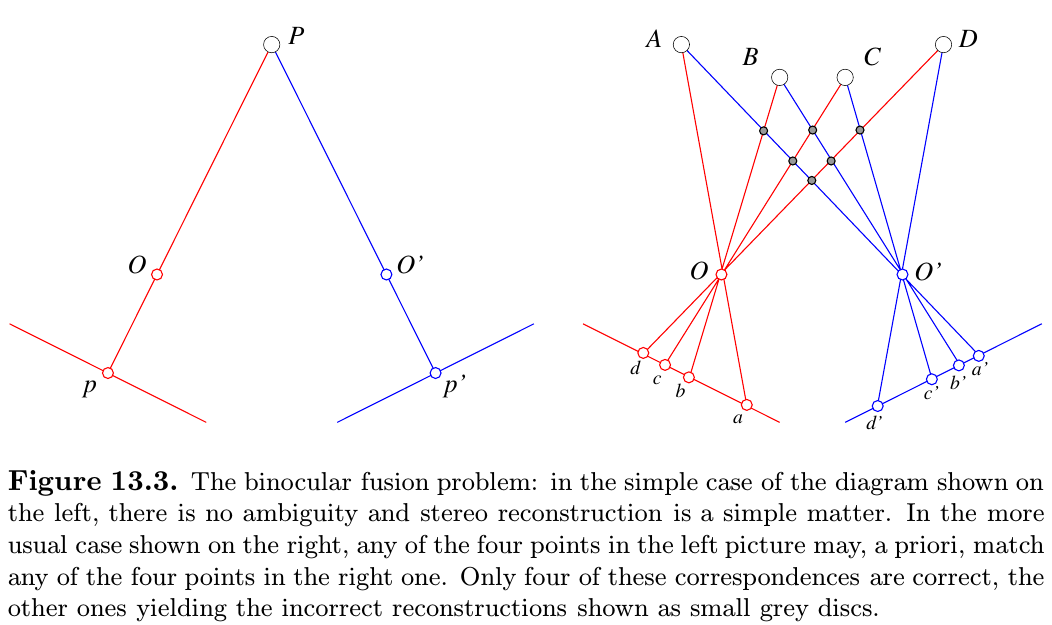
\includegraphics{img/binocular_fusion.png}}
\end{frame}}{\begin{frame}
  \frametitle{重建}
  \begin{eqnarray*}
    z\tmmathbf{p} & = & \mathcal{M}\tmmathbf{P}\\
    z' \tmmathbf{p}' & = & \mathcal{M}' \tmmathbf{P}
  \end{eqnarray*}
  得
  \begin{eqnarray*}
    \tmmathbf{p} \times \mathcal{M}\tmmathbf{P} & = & \tmmathbf{0}\\
    \tmmathbf{p}' \times \mathcal{M}' \tmmathbf{P} & = & \tmmathbf{0}
  \end{eqnarray*}
  即
  \begin{eqnarray*}
    ([\tmmathbf{p}]_{\times} \mathcal{M}) \tmmathbf{P} & = & 0\\
    ([\tmmathbf{p}']_{\times} \mathcal{M}') \tmmathbf{P} & = & 0
  \end{eqnarray*}
\end{frame}}{\begin{frame}
  \
  
  \
  
  \resizebox{1\columnwidth}{!}{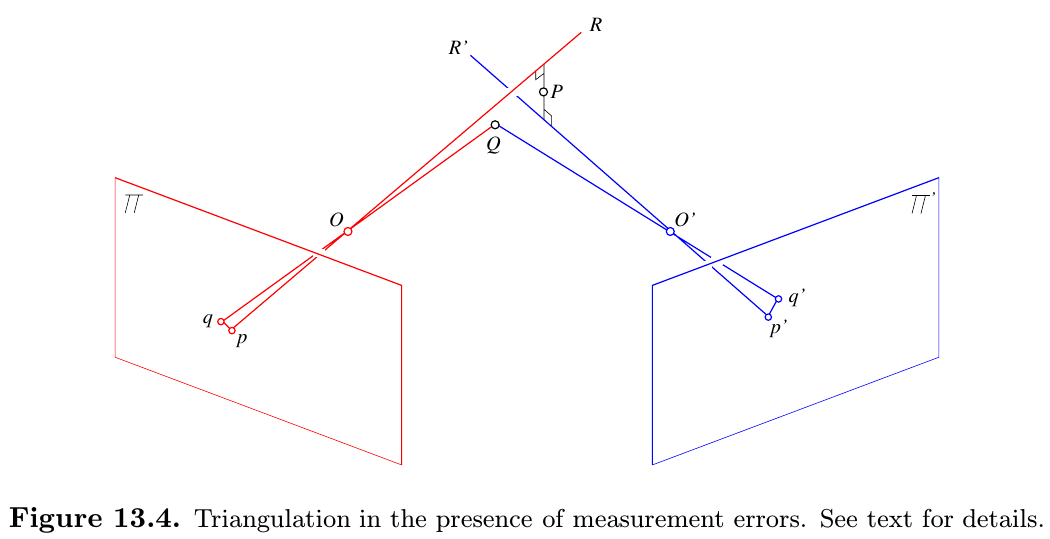
\includegraphics{img/triagulation_measurement_error.png}}
\end{frame}}{\begin{frame}
  \frametitle{图像校正}
  
  \qquad\resizebox{0.8\columnwidth}{!}{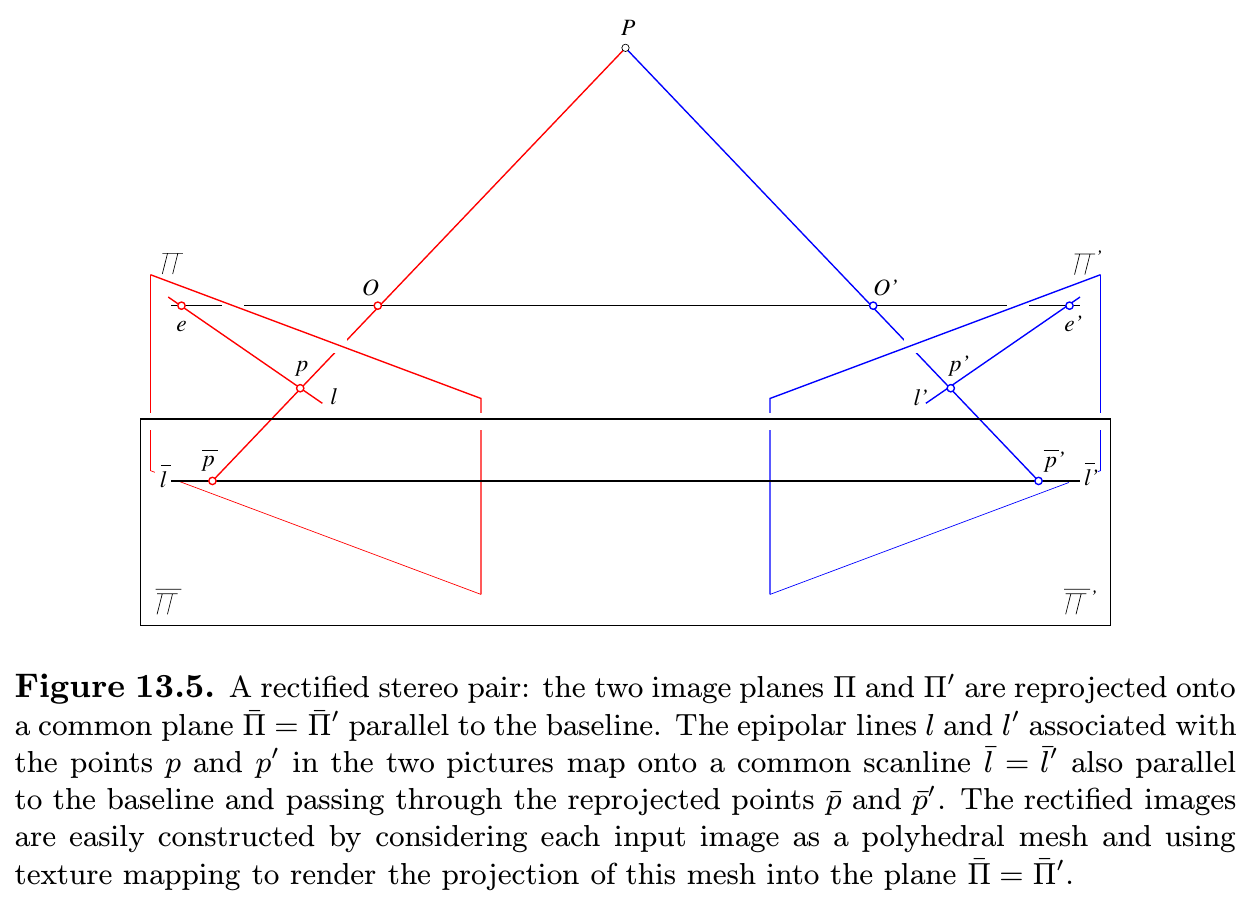
\includegraphics{img/image_rectification.png}}
\end{frame}}{\begin{frame}
  \
  
  {\hspace{4em}}\resizebox{0.8\columnwidth}{!}{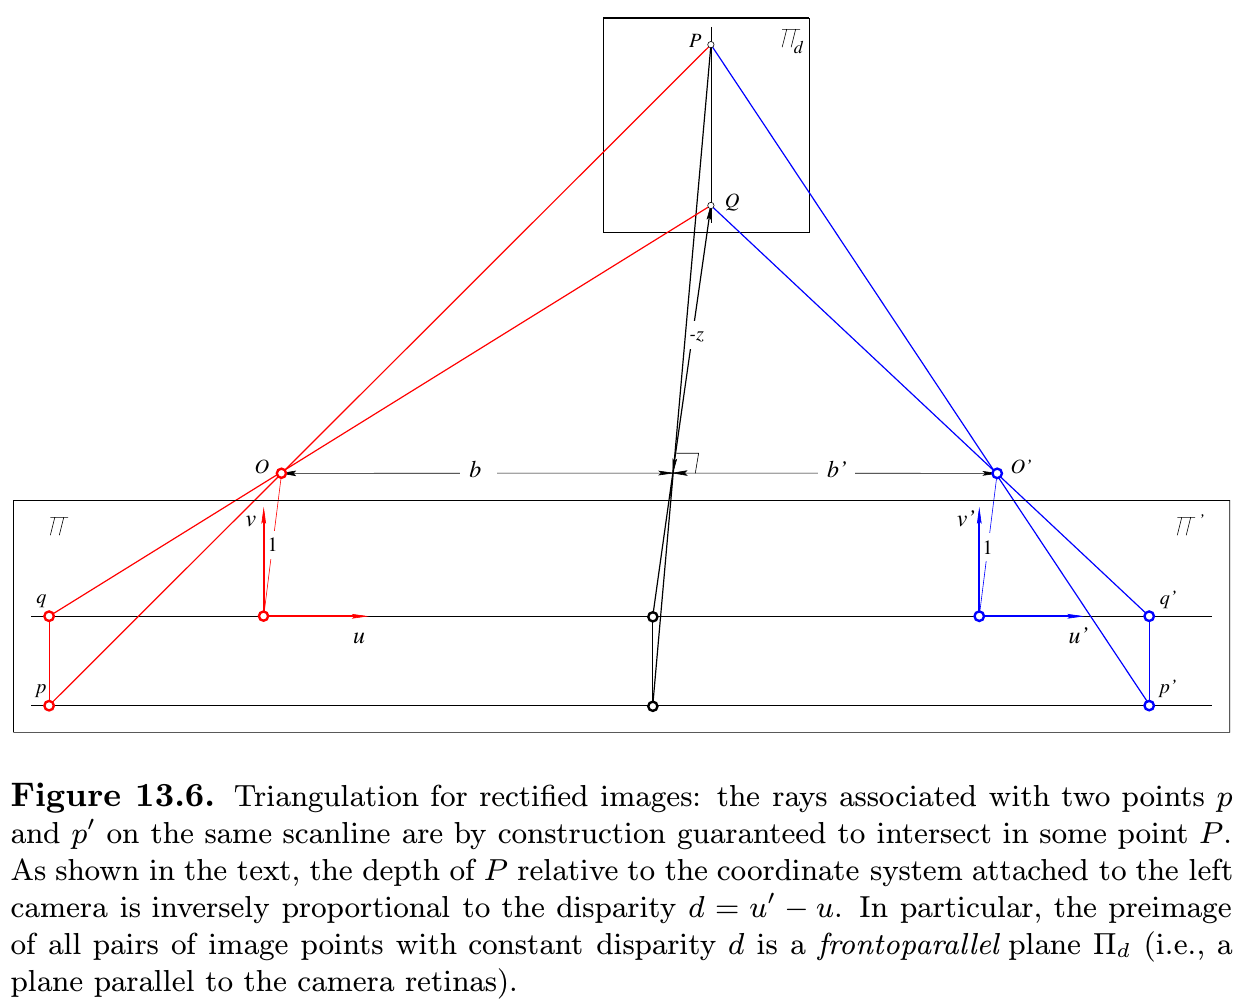
\includegraphics{img/triangulation_rectified.png}}
\end{frame}}{\frametitle{人眼立体视觉}

\resizebox{1\columnwidth}{!}{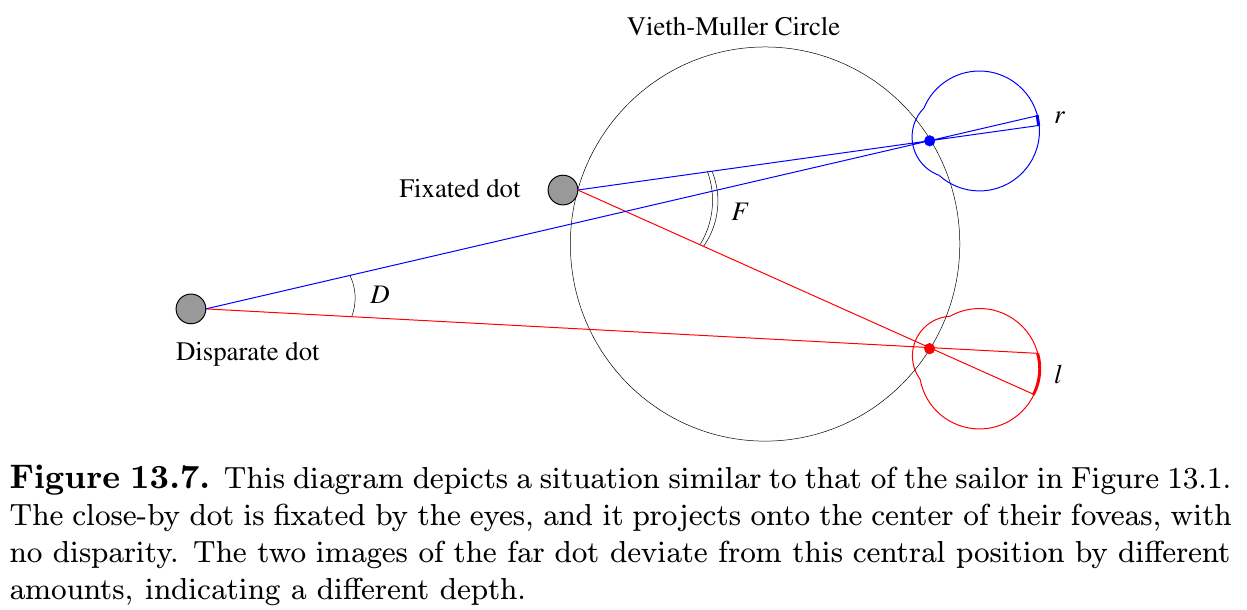
\includegraphics{img/Vieth_Muller_Circle.png}}}{\begin{frame}
  \frametitle{随机点体视图}
  
  \resizebox{1\columnwidth}{!}{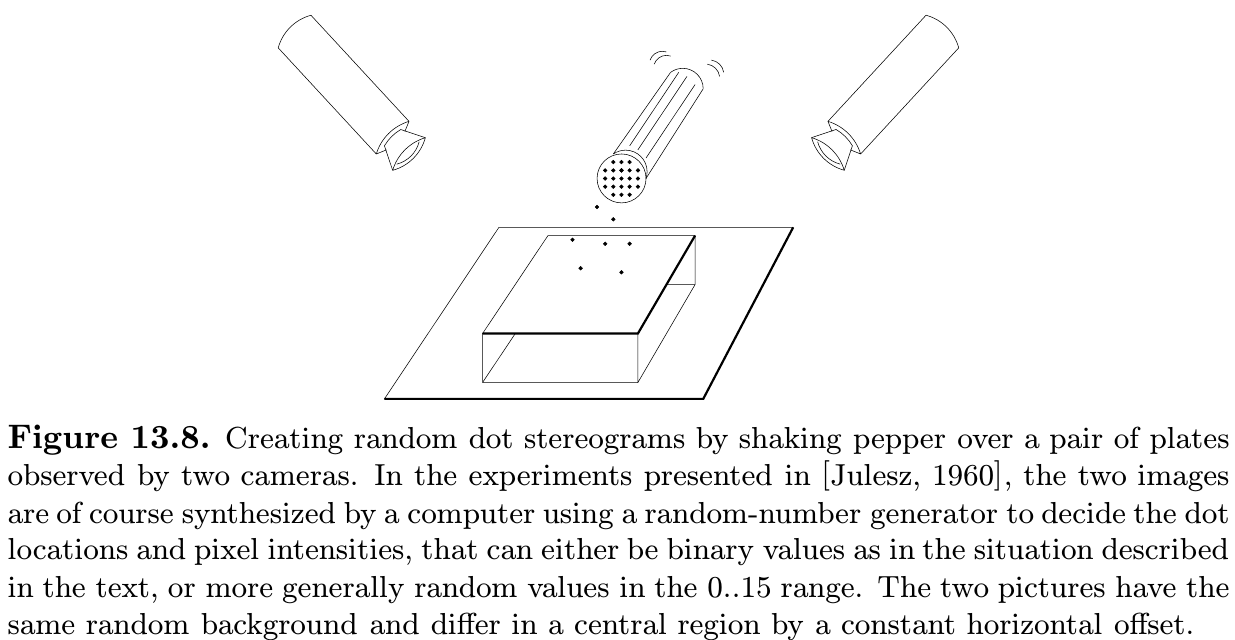
\includegraphics{img/shaking_pepper.png}}
\end{frame}}{\begin{frame}
  \frametitle{ Marr-Poggio algorithm}
  
  \resizebox{1\columnwidth}{!}{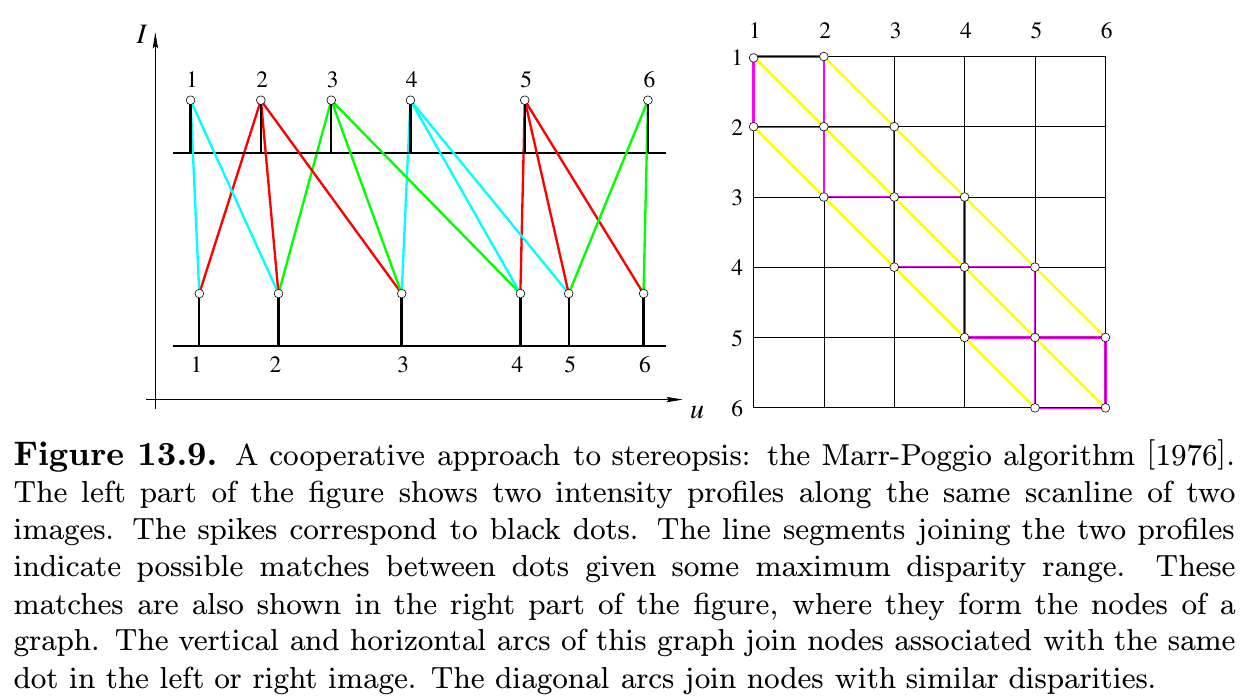
\includegraphics{img/Marr_Poggio_algorithm.png}}
\end{frame}}{\begin{frame}
  \frametitle{随机点体视图融合}
  
  \resizebox{1\columnwidth}{!}{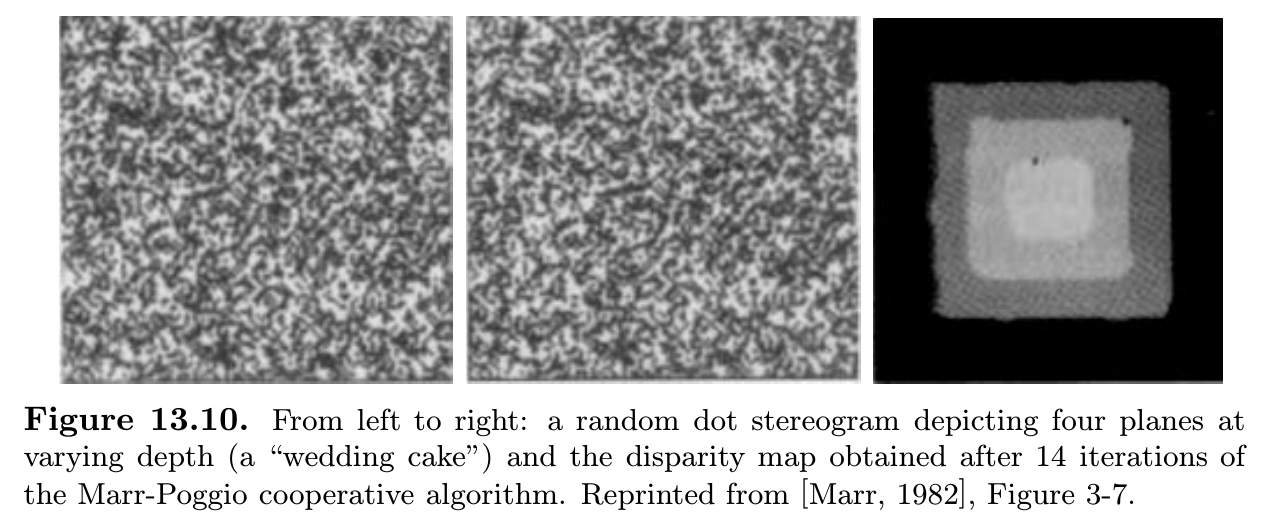
\includegraphics{img/random_stereogram_fusion.png}}
\end{frame}}{\begin{frame}
  \frametitle{相关法找对应点}
  
  {\hspace{3em}}\resizebox{0.7\columnwidth}{!}{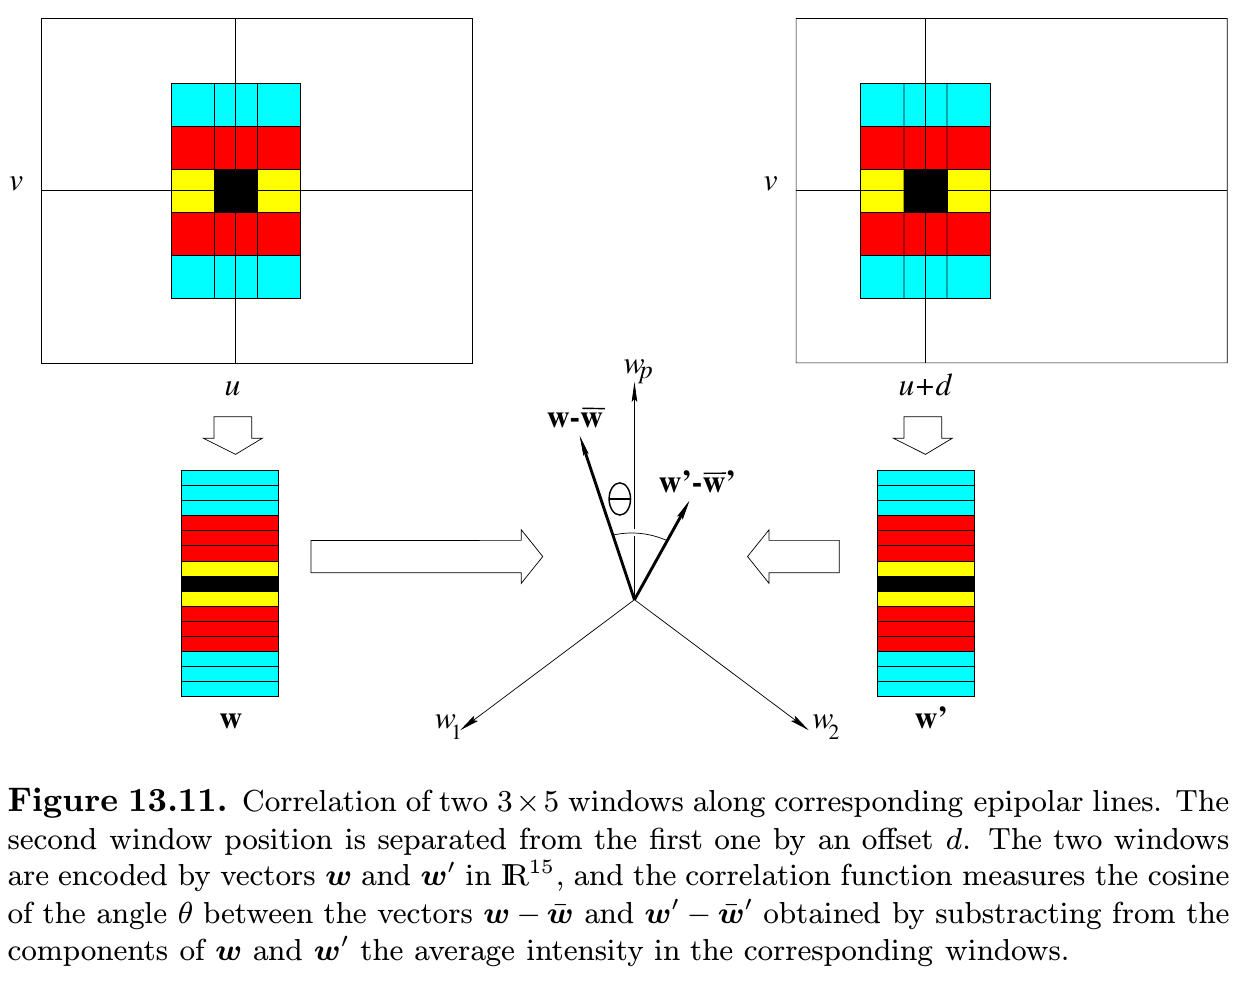
\includegraphics{img/correlation.png}}
\end{frame}}{\begin{frame}
  \frametitle{透视缩小}
  
  \resizebox{1\columnwidth}{!}{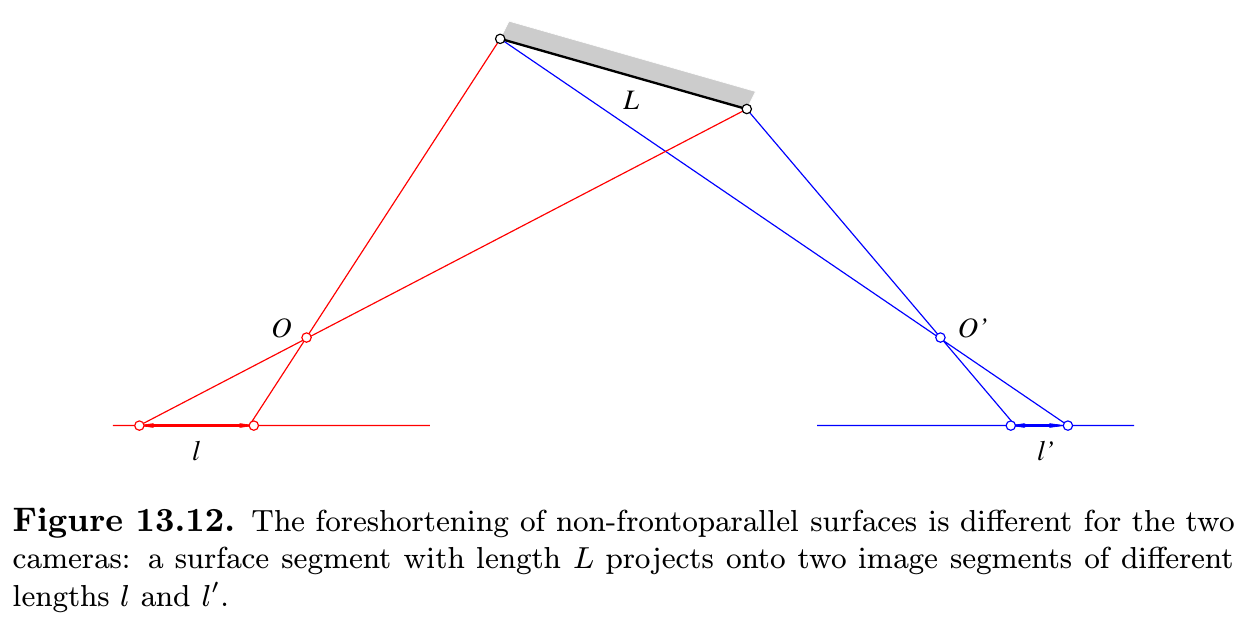
\includegraphics{img/foreshortening.png}}
\end{frame}}{\begin{frame}
  \frametitle{边缘匹配}
  
  \qquad\resizebox{0.8\columnwidth}{!}{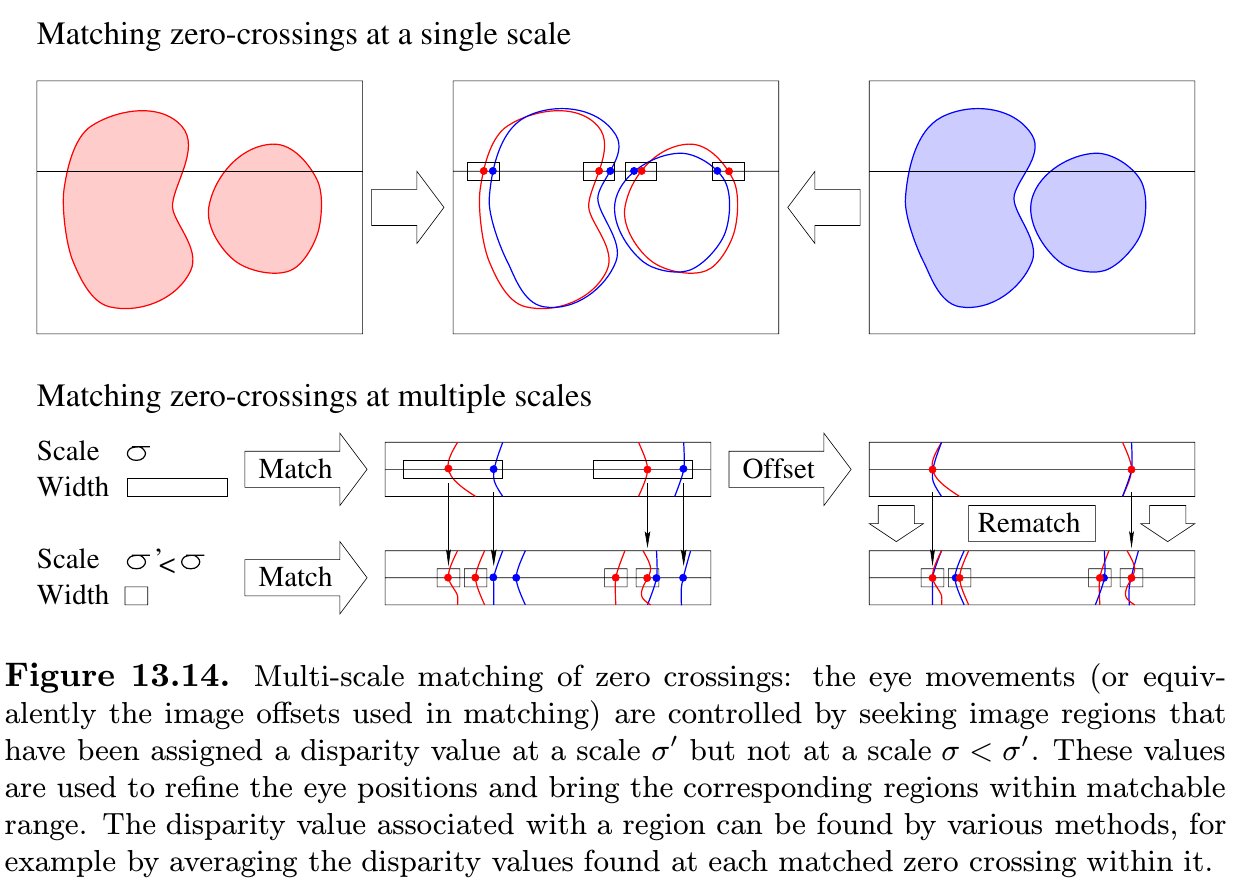
\includegraphics{img/matching_edge.png}}
\end{frame}}{\begin{frame}
  \frametitle{次序约束}
  
  \resizebox{1\columnwidth}{!}{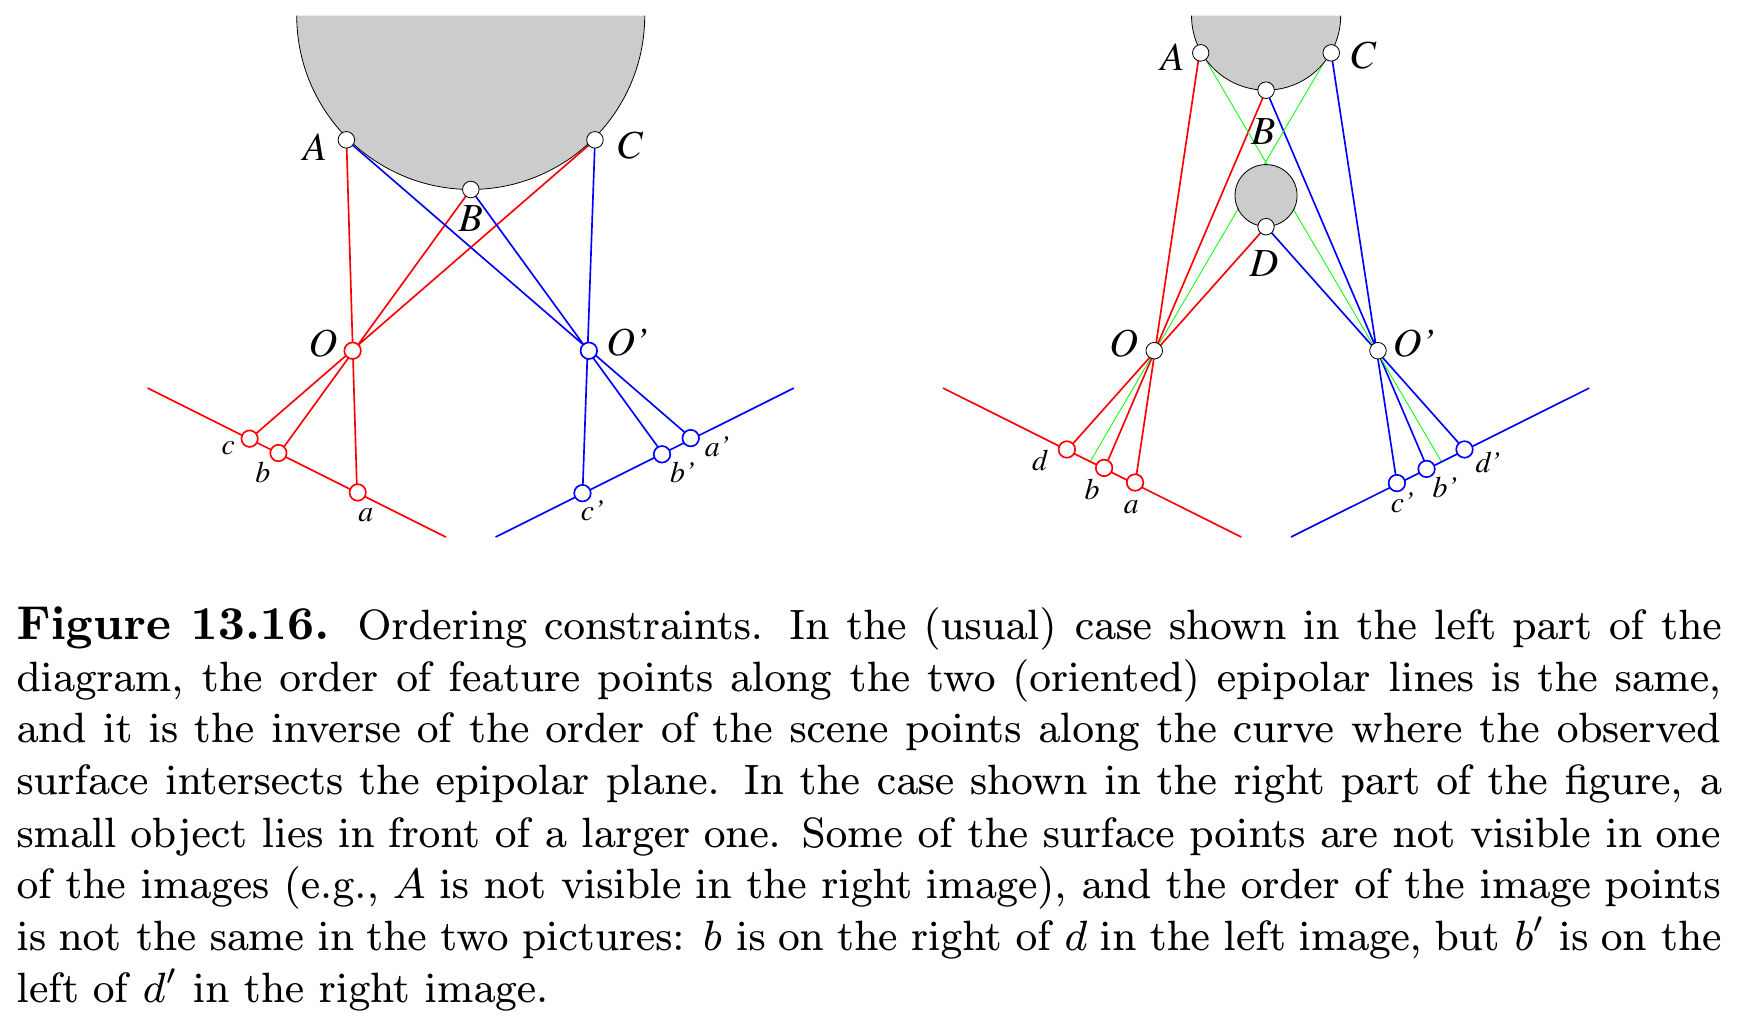
\includegraphics{img/ordering_constraints.png}}
\end{frame}}{\begin{frame}
  \frametitle{动态规划}
  
  \resizebox{1\columnwidth}{!}{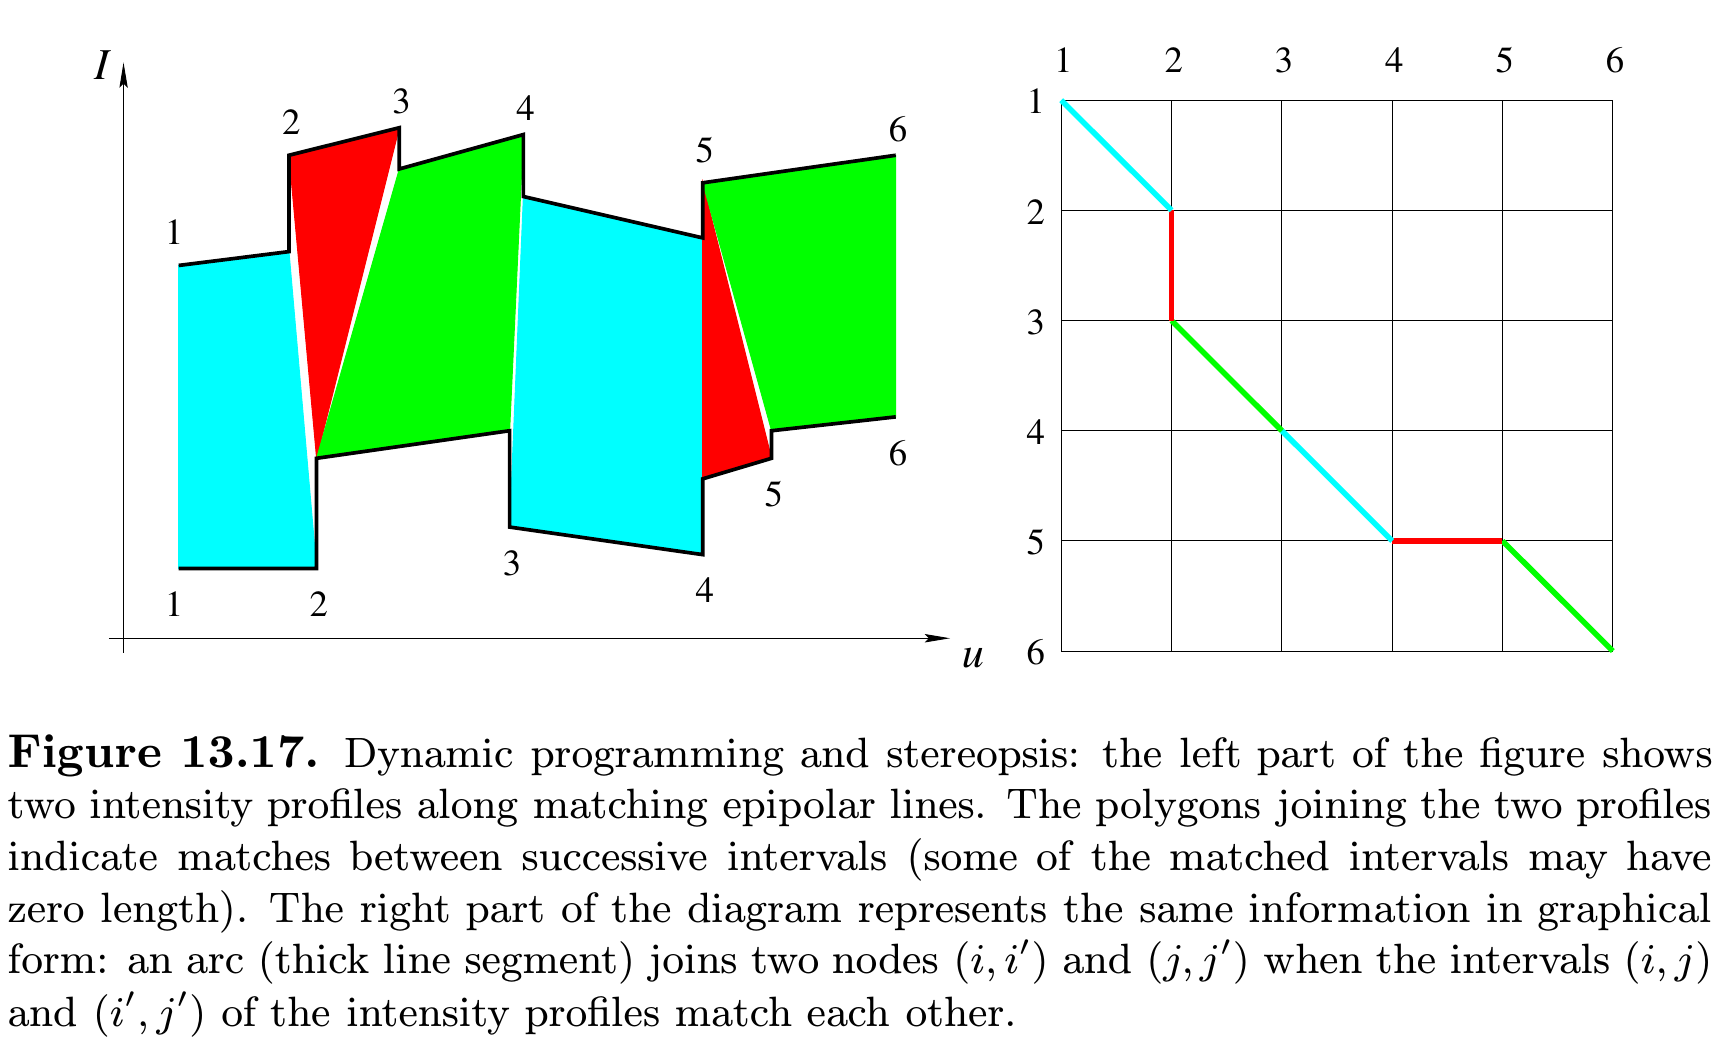
\includegraphics{img/dynamic_programming.png}}
\end{frame}}{\begin{frame}
  \frametitle{Dynamic Programming}
  \begin{itemizedot}
    \item  m, n : edge points, (the endpoints of the scanlines are included.)
    
    \item Inferior-Neighbors(k, l): neighbors (i, j) of t (k, l) i {\leq} k, j
    {\leq} l,
    
    \item Arc-Cost(i, j, k, l): \ cost of matching the intervals (i, k) and
    (j, l).
    
    \item C(1, 1): \ should be initialized with a value of zero.
  \end{itemizedot}
  \tmfoldedstd{\% Loop over all nodes (k, l) in ascending order.}{for k = 1 to
  m do
  
  {\hspace{3em}}for l = 1 to n do
  
  {\hspace{8em}}\% Initialize cost C(k, l) and backward pointer B(k, l).
  
  {\hspace{8em}}C(k, l) {\leftarrow} +{\infty}; B(k, l) {\leftarrow} nil;
  
  \tmfoldedstd{{\hspace{7em}}\% Loop over all inferior neighbors (i, j) of (k,
  l).}{{\hspace{7em}}for (i, j) {\in} Inferior-Neighbors(k, l) do
  
  {\hspace{7em}}\% Compute cost, update backward pointer
  
  {\hspace{11em}}d {\leftarrow} C(i, j) + Arc-Cost(i, j, k, l);
  
  {\hspace{11em}}if d < C(k, l)
  
  {\hspace{11em}}then C(k,l){\leftarrow}d; B(k,l){\leftarrow}(i, j)
  
  {\hspace{11em}}endif;
  
  {\hspace{7em}}endfor;}
  
  \
  
  {\hspace{3em}}endfor;
  
  endfor;}
  
  \tmfoldedstd{\% Construct optimal path by following backward pointers from
  (m, n).}{P {\leftarrow} \{(m, n)\};
  
  (i, j) {\leftarrow} (m, n);
  
  while B(i, j) != nil do
  
  {\hspace{3em}}(i, j) {\leftarrow} B(i, j);
  
  {\hspace{3em}}P {\leftarrow} \{(i, j)\} {\cup} P
  
  endwhile.}
  
  \
  
  \ 
\end{frame}}{\begin{frame}
  \frametitle{三目立体视觉}
  
  \resizebox{1\columnwidth}{!}{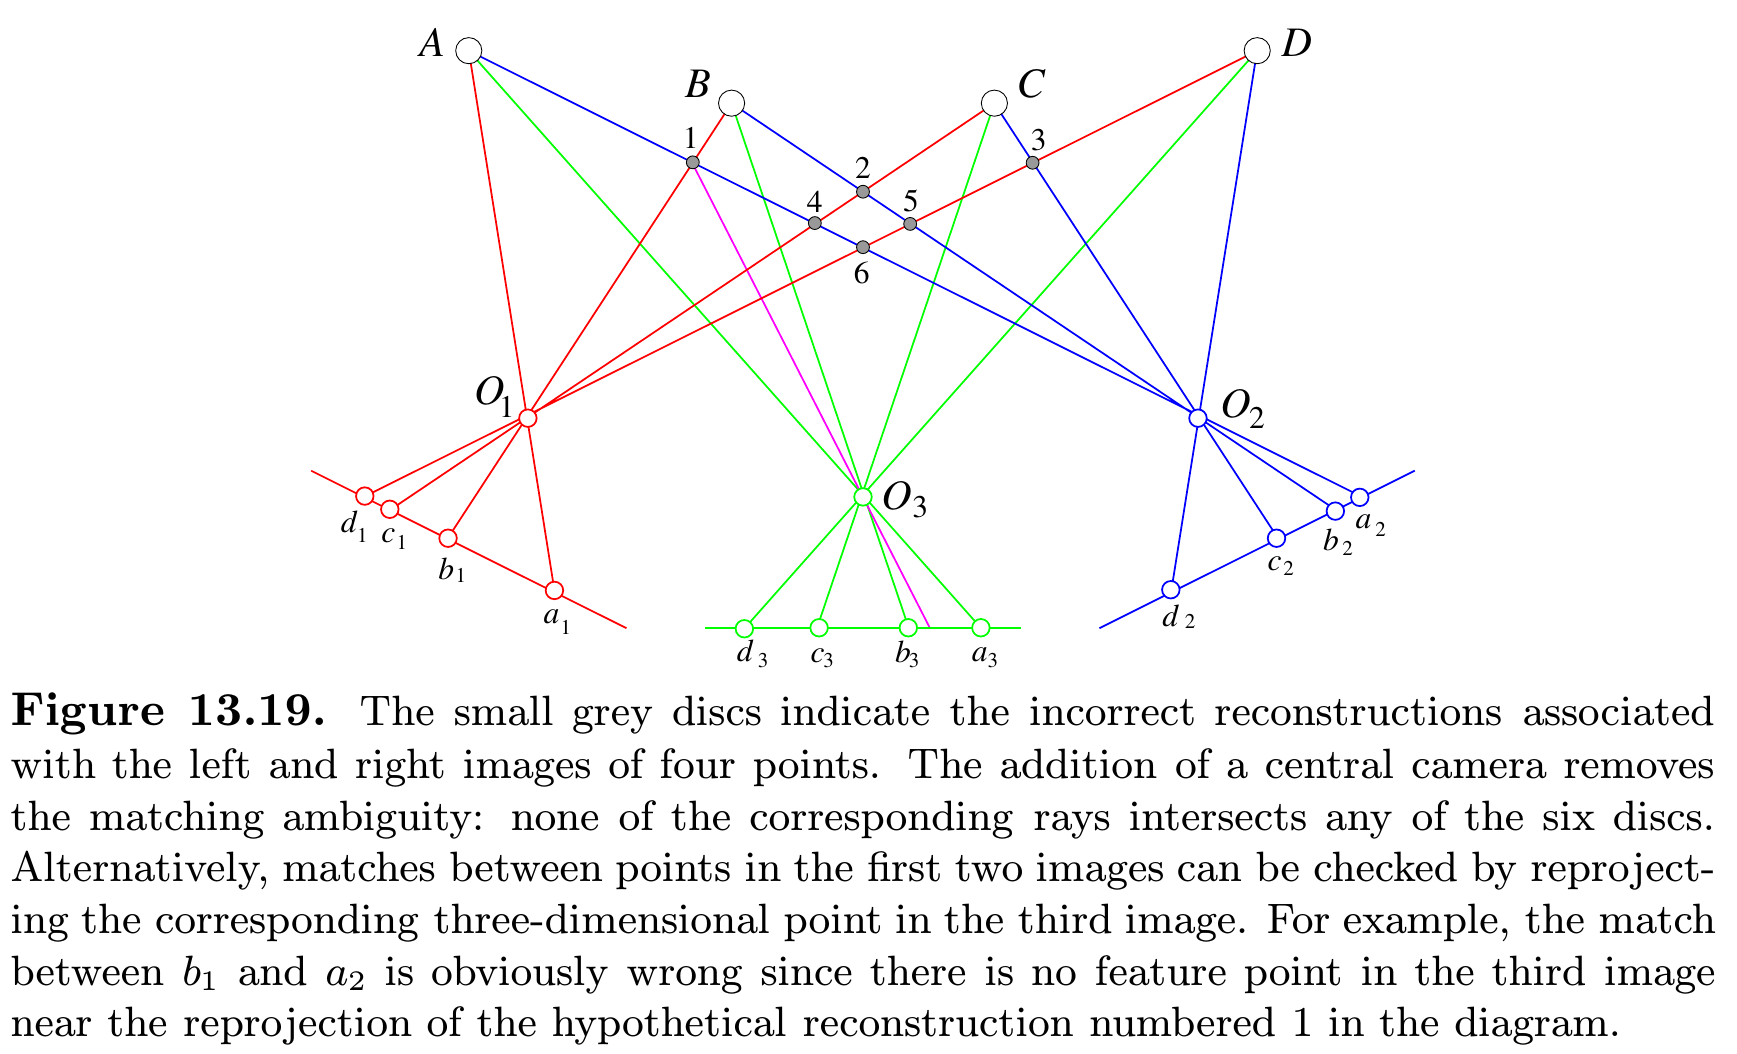
\includegraphics{img/trinocular_sterero.png}}
\end{frame}}{\begin{frame}
  \frametitle{曲线切线预测}
  
  \resizebox{1\columnwidth}{!}{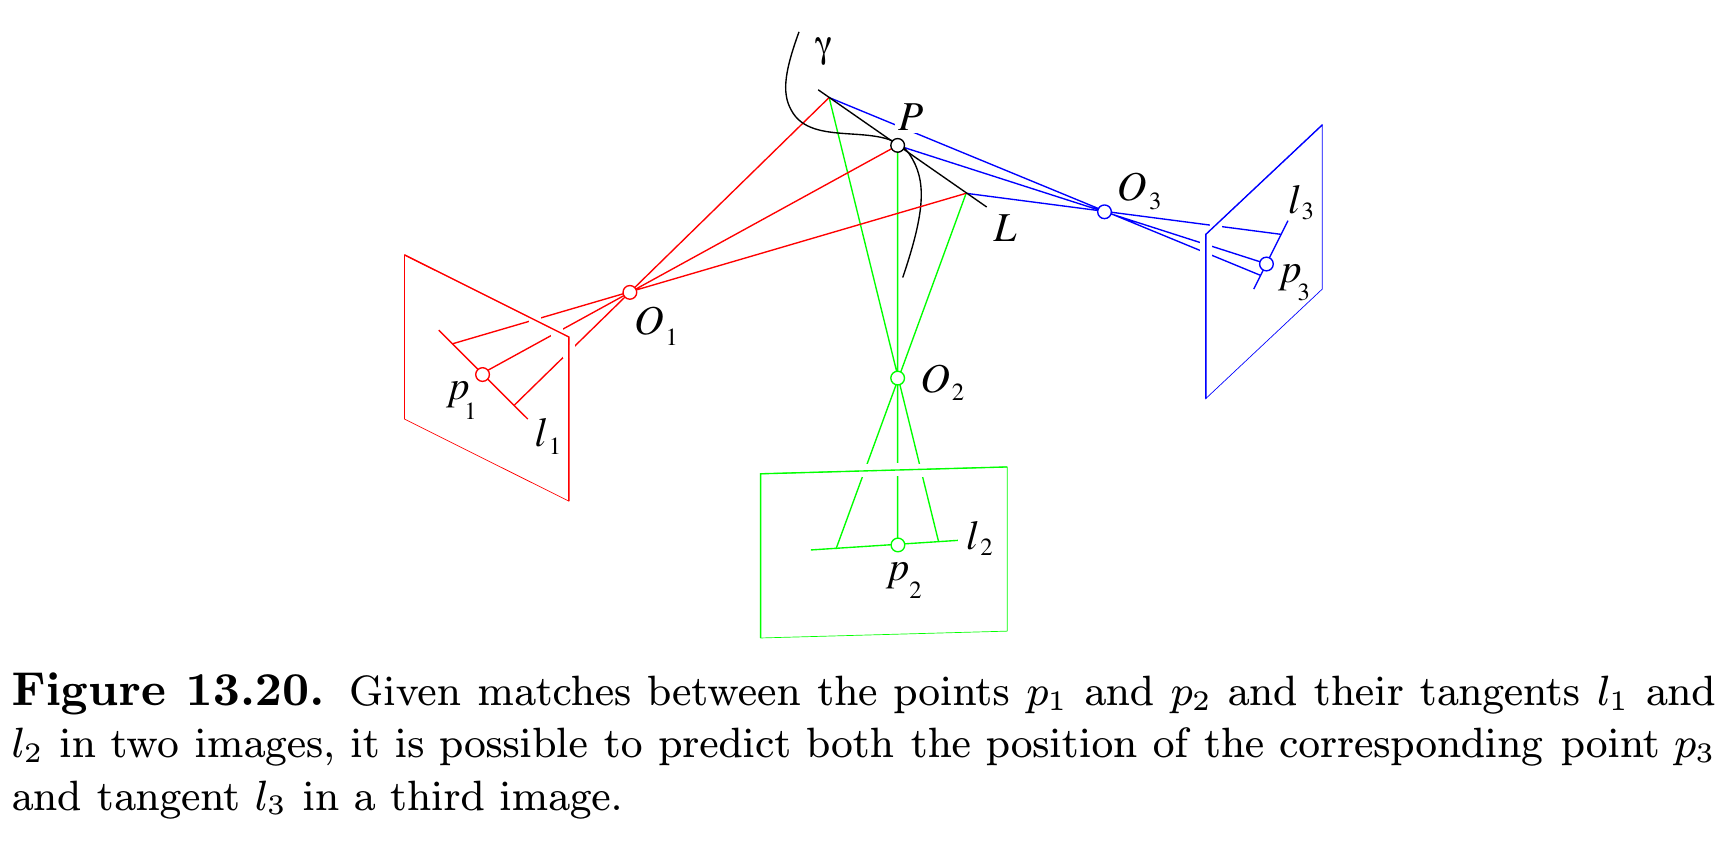
\includegraphics{img/from_p1_p2_to_p3.png}}
  
  \tmfoldedstd{ Note}{\begin{eqnarray*}
    \tmmathbf{l}_1 & \propto & \left(\begin{array}{c}
      \tmmathbf{l}_2^T \mathcal{G}_1^1 \tmmathbf{l}_3\\
      \tmmathbf{l}_2^T \mathcal{G}_1^2 \tmmathbf{l}_3\\
      \tmmathbf{l}_2^T \mathcal{G}_1^3 \tmmathbf{l}_3
    \end{array}\right)\\
    \mathcal{G}_1^i & = & \tmmathbf{t}_2 \tmmathbf{R}_3^{i \nospace T}
    -\tmmathbf{R}_2^i \tmmathbf{t}_3^T \qquad i = 1, 2, 3
  \end{eqnarray*}}
\end{frame}}}

\end{document}
